\section{Bubble sort}
El siguiente algoritmo que se ha anañizado ha sido la ordenacion de la burbuja o bubble sort, la cual como demostraremos a continuacion es de orden $O(n^{2})$, y se han realizado pruebas con distintas implementaciones asi como en distintos escenarios, como son mejor y peor caso.

El código del Bubble sort es el siguiente:

\begin{lstlisting}
  void ordenar(int *v, int n) {
    bool cambio=true;
    for (int i=0; i<n-1 && cambio; i++) {
      cambio=false;
    for (int j=0; j<n-i-1; j++)
      if (v[j]>v[j+1]) {
        cambio=true;
        int aux = v[j];
        v[j] = v[j+1];
        v[j+1] = aux;
      }
    }
  }

\subsection{Eficiencia teorica}

\begin{equation}
  T(n)=\sum_{i=0}^{n-1}(\sum_{j=0}^{n-i-1}(4+max(3+4+3,0)))=14n^{2}
\end{equation}

Por lo que sabemos que el algoritmo tiene una $O(n^{2})$.


\subsection{Eficiencia empirica}
Para demostrar que en efecto el tiempo de ejecucion de nuestro algoritmo evoluciona conforme nos ha indicado la eficiencia teorica, se hicieron varias ejecuciones con dicho algoritmo para diferentes tamaños de entradas, obteniendo la siguiente grafica:

\begin{figure}[H]
  \centering
  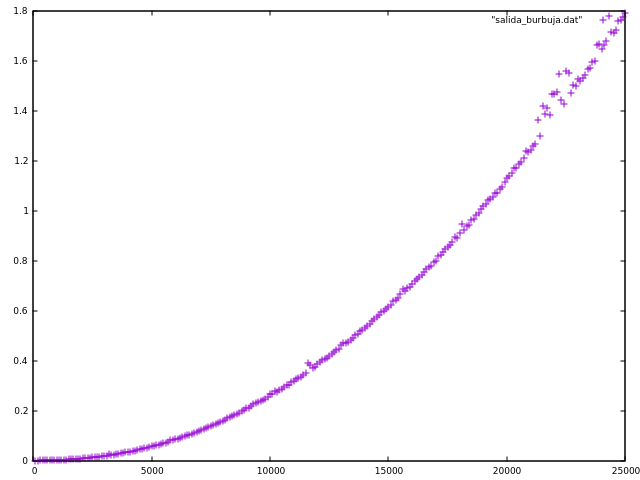
\includegraphics[width=0.5\textwidth]{./Imagenes/burbuja_pela.png}
  \caption{Grafica con los tiempos de ejecucion del algoritmo bubble sort}
\end{figure}


\subsection{Ajuste de la grafica con $f(x)=x^{2}$}
Si procedemos a comprobar como se ajusta la eficiencia teorica con la grafica obtenida en el apartado anterior veremos como efectivamente se corresponde a la perfección con una gráfica de una funcion polinomica de grado 2, lo cual nos demuestra lo inficiente de este algoritmo en cuanto el tamaño de las entradas crece. La grafica es la que se muestra a continuación:

\begin{figure}[ht]
  \centering
  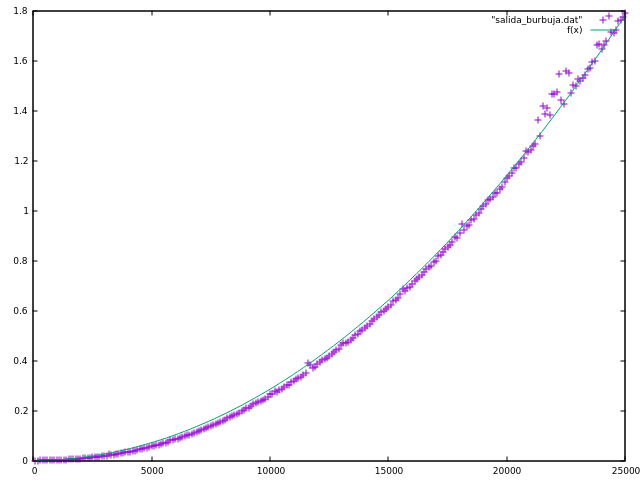
\includegraphics[width=0.5\textwidth]{./Imagenes/burbuja_ajustada.png}
  \caption{Ajuste de la salida de bubble sort con $f(x)=x^{2}$}
\end{figure}

\subsection{Influencia del proceso de compilacion en la eficiencia empirica de un algoritmo}
Como hemos comprobado en el anterior apartado, en efecto los tiempos de ejecucion del algoritmo en cuestion crecen en la medida que predijimos en el calculo teórico de la eficiencia, pero se nos plantea la duda de en que medida el proceso de compilación de nuestro programa, con lo cual se procedio a compilar el mismo programa con el que se habian obtenido los datos de las graficas anteriores, pero ahora se compilo usando el flag -O3 aplicando asi el compilador un mayor grado de optimización a las instrucciones maquina generadas. Tras enfrentar la grafica del programa optimizado a la grafica anterior se obtuvo los siguientes resultados que a continuación analizaremos:

\begin{figure}[H]
  \centering
  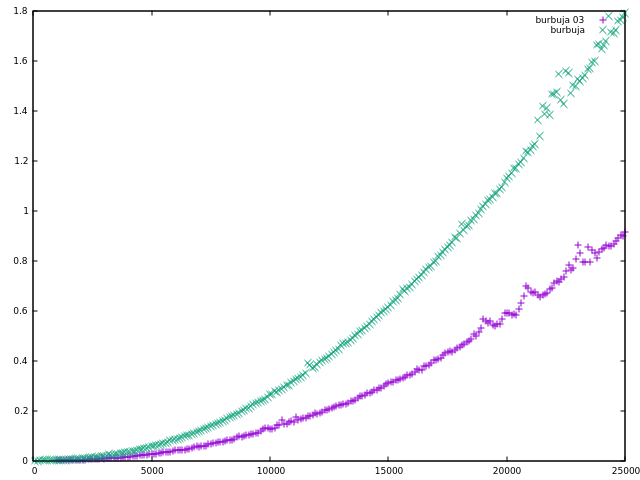
\includegraphics[width=0.5\textwidth]{./Imagenes/burbuja_vs_eficaz.png}
  \caption{Algoritmo sin optimizavion vs algoritmo con optimizacion}
\end{figure}

Si nos fijamos en la anterior grafica se ve como el proceso de compilacion si que afecta y mucho a las constantes ocultas, que afectan a la eficiencia de nuestro algoritmo, ya que dos implementaciones, la primera de ellas de orden $2*n^{2}$ y la segunda de orden $100*n^{2}$ son de orden $O(n^{2})$, pero como el lector adivinará la primera es mucho mejor ya que su factor multiplicativo es mucho menor, asi observamos que la segunda version en el maximo tamaño de entradas es 1 segundo mas rapida (en otros PC's estos tiempor podrian variar), y esta tendencia se mantendría hasta el infinito.

\subsection{Mejor y Peor Caso}
%subtitle{Ejercicio 4}

Cuando ejecutamos nuestros programas, estos trabajan sobre datos que cabe esperar que estén desordenados, pero se puede dar el caso en el que estos datos tengan una pecularidad que afecte al tiempo de ejecución.

\subsubsection{Mejor caso}

En este algoritmo, el mejor caso es que el vector de datos esté ordenado, ya que que no tiene que intercambiar ningún elemento, por lo que el tiempo de cómputo es menor.

En la siguiente gráfica, tras hacer pruebas con distintos tamaños de entrada, se ve el tiempo (eje Y) en relación a la entrada de datos (eje X).

\begin{figure}[ht]
  \centering
  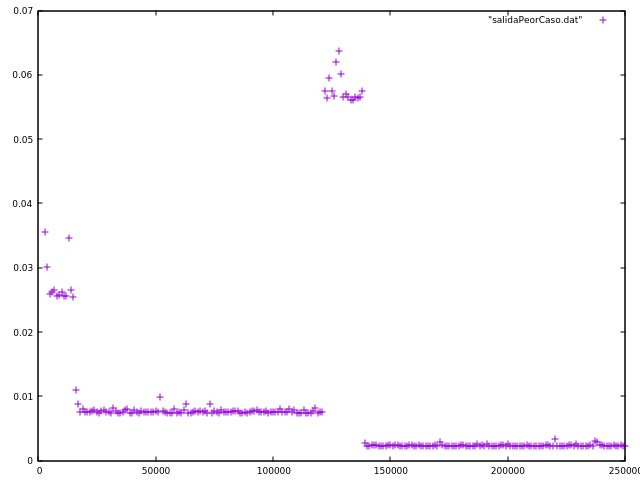
\includegraphics[width=0.5\textwidth]{./Imagenes/mejorCaso.png}
  \caption{Datos de la salida del algoritmo de ordenación por burbuja}
\end{figure}

Donde se aprecia que con independencia del tamaño del vector que haya que ordenar el tiempo es practicamente constante, ya que se podria ajustar perfectamente a una recta, si obviamos las variaciones debidas a procesos del sistema operativo y otros aspectos que siempre afectan a estos analisis.

\subsubsection{Peor caso}

Este caso se da si el vector de datos de entrada está ordenado inversamente, ya que en cada iteracción habrá que hacer un intercambio, por lo que el tiempo de cómputo es mayor.

Observamos en la siguiente gráfica la compración entre el tiempo (eje Y) respecto del tamaño de datos de la entrada (eje X) del mejor y peor caso.

\begin{figure}[ht]
  \centering
  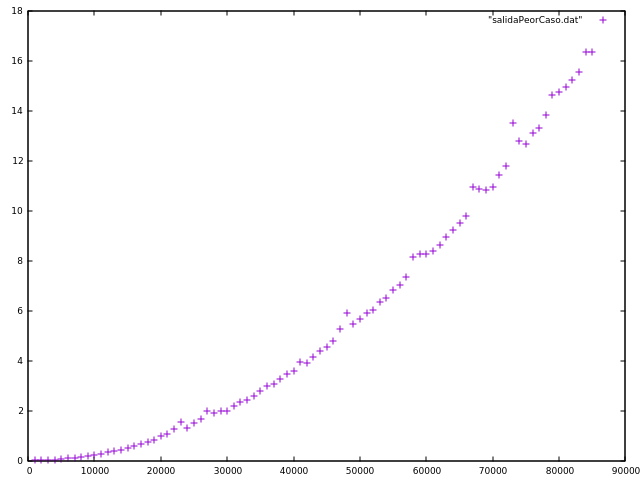
\includegraphics[width=0.5\textwidth]{./Imagenes/peorCaso.png}
  \caption{Peor caso en el algoritmo bubble sort}
\end{figure}


A continuacion se muestran las tres graficas enfrentadas, caso promedio, peor y mejor caso:

\begin{figure}[ht]
  \centering
  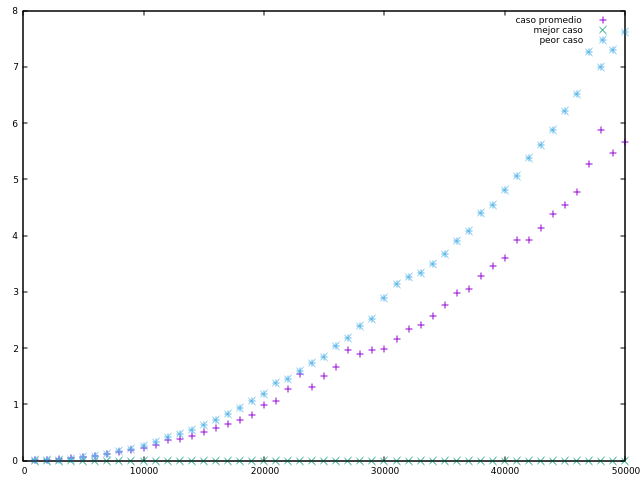
\includegraphics[width=0.5\textwidth]{./Imagenes/casosEnfrentados.png}
  \caption{Casos enfrentados}
\end{figure}
